\section{Practice - implementation as REST Service}
The project have 3 main goal tool for transportation modelling and web application for it. So we had to make REST service. This service is based on python micro-framework Flask. In Fig. \ref{img.b} you can see all backend environment.

\begin{figure}
\centering
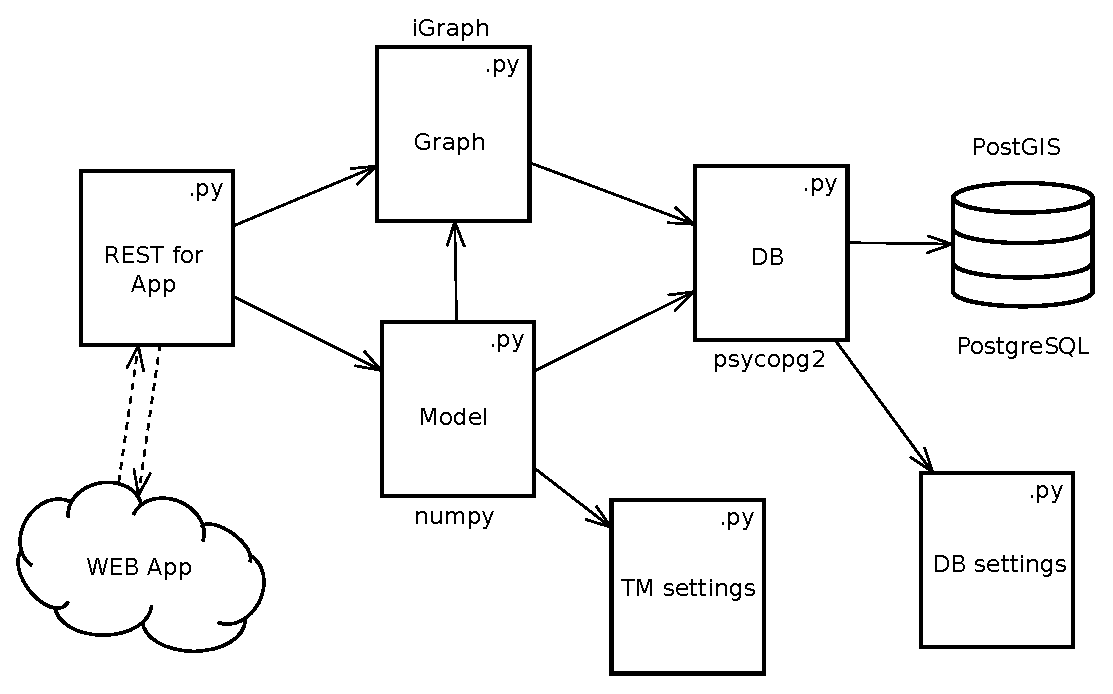
\includegraphics[width=15cm]{img/c01-transp-model/backend.eps}
\caption{Backend (REST)}
\label{img.b}
\end{figure}

Recompute traffic take a lot of time, so REST must be asynchronous. In our approach we made two service. First service start compute and second return progress.

Example:
\begin{verbatim}
/api/compute_traffic

{"status": "ok", "result": "calculation began"}

/api/compute_traffic_progress

{"status": "ok", "result": {"progress": 34, "isrun": true}}
\end{verbatim}